\chapter{TỔNG QUAN}
\textbf{
\section{Màu sắc răng}}
\vspace{-5pt}
\subsection{Màu sắc răng tự nhiên}
\vspace{-5pt}
\qquad Màu sắc là đặc tính ba chiều không gian được xác định bởi: tông màu, độ đậm nhạt của màu, độ sáng tối của màu. Khi đánh giá màu răng bình thường: tông màu do ngà quyết định, độ sáng tối do men quyết định.\cite{sachchuarangnoinha}\par
\vspace{-5pt}
\subsection{Các thành phần chi phối màu sắc}
\par
\vspace{-5pt}
\qquad Có ba yếu tố ảnh hưởng đến màu sắc bao gồm: tông màu (Hue), độ bão hoà (Saturation/Chroma), giá trị màu (Value/Brightness).\cite{TruongDinhKhoi}\par
\vspace{-5pt}
\quad \textit{Hue:} là một trong những đặc tính chính của màu sắc thể hiện mức độ khác nhau của màu sắc. Hue đóng vai trò là màu căn bản thường là tổ hợp 12 màu đậm nhạt trên vòng tuần hoàn màu - Color Wheel.\cite{TruongDinhKhoi}\par
\vspace{-5pt}
\quad \textit{Saturation/Chroma:} là độ rực rỡ của màu sắc hoặc độ bão hoà của màu đề cập đến cường độ của màu sắc trong hình ảnh. Khi độ bão hoà tăng lên, màu sắc được đẩy mạnh hơn mang đến màu sắc sống động, phong phú và tươi sáng. Ngược lại, khi độ bão hoà giảm xuống, màu sắc có vẻ nhợt nhạt hơn.\cite{TruongDinhKhoi}\par
\vspace{-5pt}
\quad \textit{Value/Brightness:} Còn được gọi là giá trị màu, chỉ độ sáng tối của màu sắc, cũng có thể là một thước đo ánh sáng về màu sắc. Theo đó, giá trị của màu sắc được thay đổi bằng cách thêm màu trắng hoặc đen vào màu sắc.\cite{TruongDinhKhoi}

%chèn hình ảnh yếu tố chi phối màu sắc răng ở đây ạaa
\begin{figure}[h]
\centering
    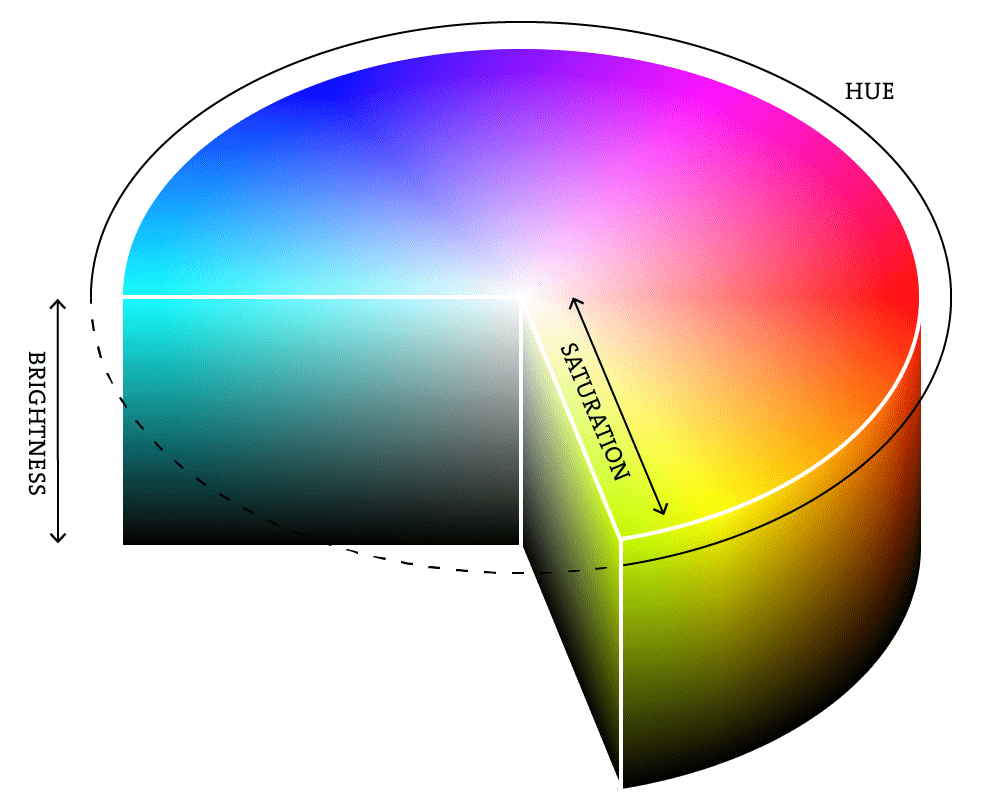
\includegraphics[width=0.6\columnwidth]{pictures/nguyen-tac-phoi-mau-18.png}
    \caption{Ba yếu tố chi phối màu sắc răng}
    \label{fig:nguyen-tac-phoi-mau}
\end{figure}

\textbf{
\section{Các yếu tố ảnh hưởng đến so màu trong nha khoa}}
\vspace{-5pt}
\subsection{Ánh sáng}
\vspace{-5pt}
\qquad Không thể so màu chính xác khi thiếu hoặc thừa ánh sáng, ánh sáng khi so màu răng phụ thuộc vào nguồn sáng và cường độ sáng khi ánh sáng chiếu đến vật thể so màu và phản xạ lại mắt người so màu.\par
\vspace{-5pt}
\quad Cường độ ánh sáng (độ sáng) ảnh hưởng đến đường kính giãn đồng tử của người so màu, ảnh hưởng đến kết quả so màu. Cường độ thích hợp để so màu trong nha khoa là vừa đủ để đồng tử giãn và ánh sáng phản xạ từ vật thể tập trung vào hố thị giác của võng mạc, từ 1000-2000 lux, được xác định bằng dụng cụ ánh sáng kế.\par
\vspace{-5pt}
\quad Hiện nay, trong nha khoa thường dùng ánh sáng lý tưởng để so màu là ánh sáng hiệu chỉnh (Color-corrected light) với cường độ sáng khoảng 1000-2000 lux và nguồn màu từ 5500-6500K.\cite{TruongDinhKhoi}

%chèn ảnh bảng nhiệt độ màu K
\begin{figure}[h]
    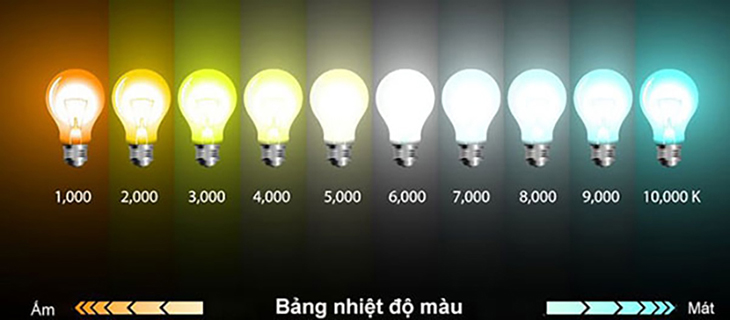
\includegraphics[width=1\columnwidth]{pictures/bảng nhiệt độ màu K.jpeg}
    \caption{Dải màu nhiệt của nguồn sáng}
    \label{fig:bảng nhiệt độ màu K}
\end{figure}

\subsection{Sự xung đột ánh sáng trong không gian so màu}
\vspace{-5pt}
\qquad Trong không gian phòng khám để so màu, nơi pha trộn giữa nhiều nguồn sáng như ánh sáng tự nhiên, ánh sáng đèn chiếu sáng, ánh sáng từ nguồn hiệu chỉnh so màu, vì vậy cần hạn chế sử dụng nhiều nguồn sáng, các nguồn sáng hỗ trợ cần có màu tương thích với màu hiệu chỉnh khi so màu hoặc màu trung tính như màu xám. Màu ánh sáng hiệu chỉnh cần thống nhất và theo chuẩn hoá hiệu chỉnh để kết quả được chính xác và tương đồng nhau. Khi màu nguồn sáng khác nhau sẽ cho ra những kết quả so màu khác nhau (hiện tượng metame so màu).\cite{TruongDinhKhoi}


%chèn ảnh màu sắc răng khác nhau 
\begin{figure}[h]
    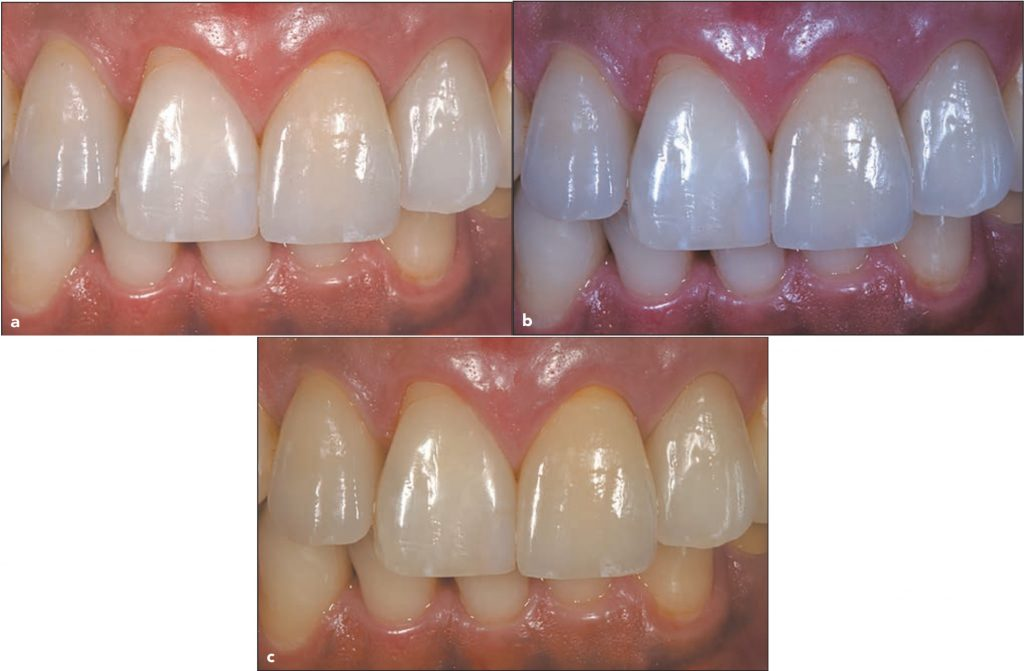
\includegraphics[width=1\columnwidth]{pictures/màu sắc răng khác nhau khi nguồn màu khác nhau.jpeg}
    \caption{Màu răng khác nhau khi nguồn màu khác nhau}
    \label{fig:màu sắc răng khác nhau khi nguồn màu khác nhau}
\end{figure}

\subsection{Hiệu ứng tương phản đồng thời trong so màu nha khoa}
\vspace{-5pt}
\qquad Tương phản đồng thời khi quan sát và so sánh màu sắc của hai hay nhiều màu cùng một lúc, khi đó mắt và não có xu hướng cân bằng và trung bình màu. Sự tương phản đồng thời ảnh hưởng bởi ba yếu tố: Cường độ sáng xung quanh (vật thể sẽ có màu tối hơn nếu vật thể xung quanh sáng hơn và ngược lại); màu của môi trường xung quanh (vật thể có xu hướng ảnh hưởng cân bằng với các màu xung quanh); độ bão hoà môi trường xung quanh (màu của vật thể có xu hướng sẫm hơn nếu môi trường ít bão hoà hơn và ngược lại).
\vspace{-5pt}
\setlength{\parskip}{-1pt}
\begin{itemize}
    \item{Tương phản đồng thời về giá trị cường độ sáng (tương phản Value)}
\end{itemize}
\vspace{-5pt}
\qquad Độ sáng của vật thể so màu bị ảnh hưởng bởi những màu nền xung quanh, màu nền tối thì vật sẽ nhìn sáng hơn và ngược lại. Mắt thích nghi với sự thay đổi màu nền từ tối sang sáng nhạy hơn so với chuyển màu nền từ sáng sang tối. Trong nha khoa, khi viền lợi bị viêm thì cổ răng sẽ sáng hơn hơn so với màu thật vì viền lợi viêm sẽ sưng và đỏ hơn so với màu lợi bình thường. Để khắc phục tương phản value thì nên chọn màu răng sáng với những bệnh nhân có tông màu sáng của răng xung quanh hoặc mô mềm xung quanh, và ngược lại.\cite{TruongDinhKhoi}

%ảnh màu sắc răng trên nền sáng tối
\begin{figure}[h]
 \centering
    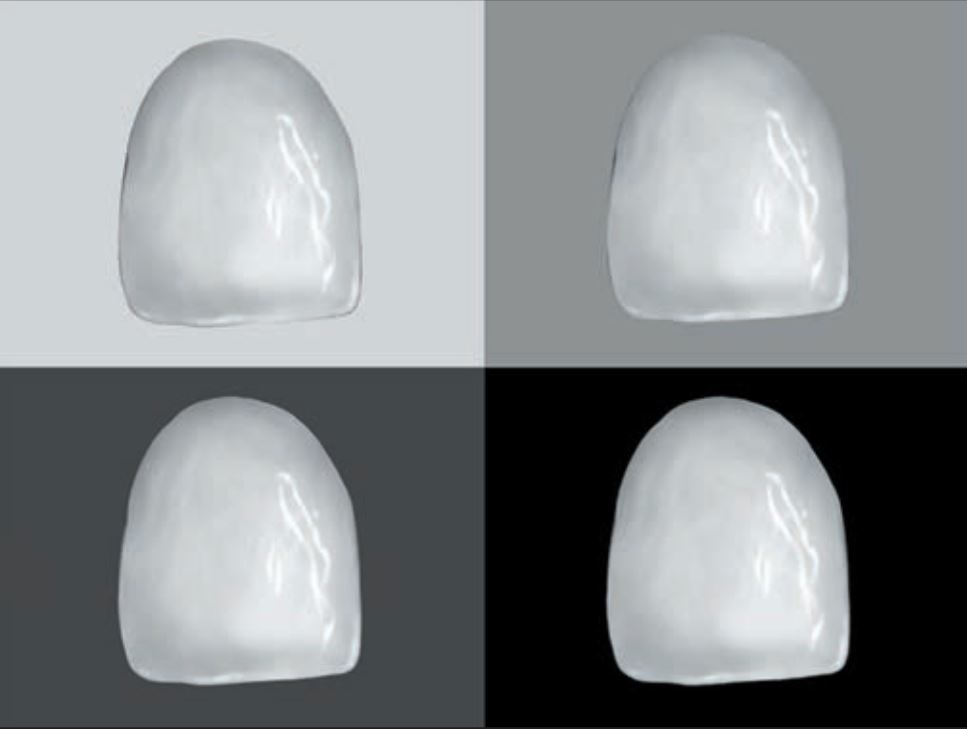
\includegraphics[width=0.8\columnwidth]{pictures/ảnh màu sắc răng trên nền sáng tối.jpeg}
    \caption{Răng sẽ sáng hơn nếu màu nền tối hơn}
    \label{fig:ảnh màu sắc răng trên nền sáng tối}
\end{figure}

\begin{itemize}
    \item{Tương phản đồng thời về màu (tương phản Hue)}
\end{itemize}
\vspace{-5pt}
\qquad Màu của vật thể có thể bị ảnh hưởng bởi màu của màu nền xung quanh. Ví dụ, răng hoặc miếng trám sẽ xanh hơn khi màu nền màu cam hoặc sẽ tím hơn nếu màu nền màu vàng. Như vậy, màu vật thể có xu hướng trung hòa với màu nền của môi trường xung quanh. Khi quan sát một màu cùng lúc với màu khác thì hue cảm nhận đầu tiên nhận được sẽ giống với màu bổ sung thứ 2, do vậy bác sĩ nên nhìn vào màu bổ sung trước khi nhìn vào màu của răng. Hầu hết màu răng đều nằm trong nhóm màu cam nên bác sĩ nên nhìn vào màu xanh dương trước khi so màu để giảm tương phản hue.\cite{TruongDinhKhoi}
\vspace{-5pt}
%chèn ảnh hue ạ


\begin{itemize}
    \item{Tương phản đồng thời về độ bão hoà (tương phản Chroma)}
\end{itemize}
\vspace{-5pt}
\qquad Độ bão hoà của vật thể sẽ lớn hơn nếu độ bão hoà của nền thấp hơn và ngược lại. Như vậy, nếu hue và chroma của vật thể càng giống với hue và chroma của màu nền thì càng khó so và phân biệt màu của vật thể đó. Trong nha khoa, không nên chọn màu nền có hue và chroma giống với hue và chroma của răng.\cite{TruongDinhKhoi}
\begin{figure}[h!]
  \centering
    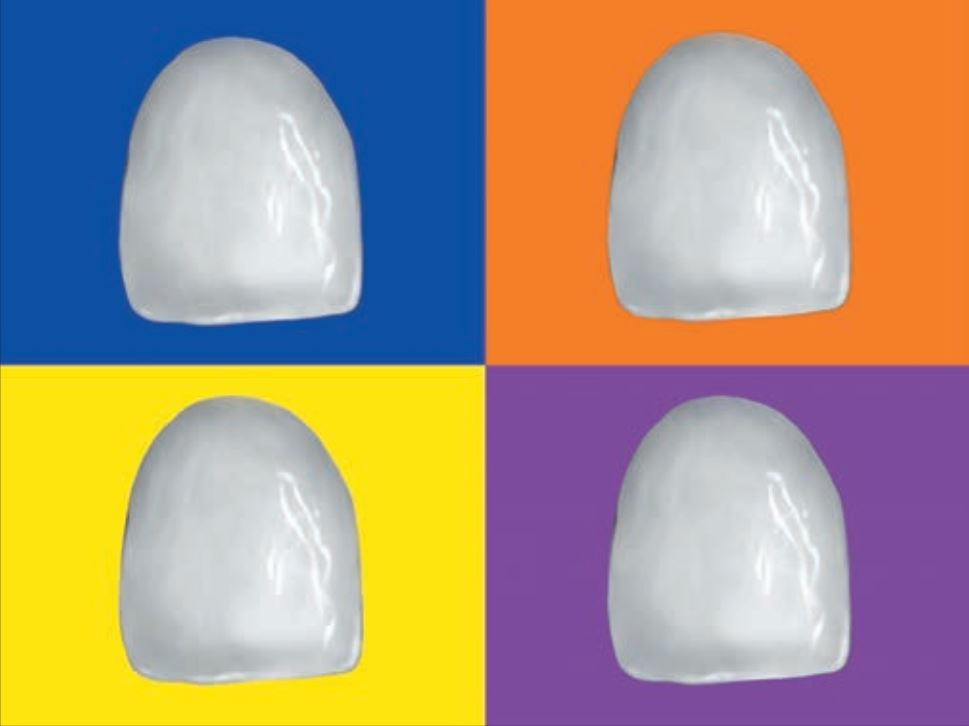
\includegraphics[width=0.6\columnwidth]{pictures/hue.jpeg}
    \caption{Răng có xu hướng trung hòa với màu nền, răng tím hơn nếu nền màu vàng, màu cam hơn nếu nền màu xanh dương, vàng hơn nếu màu nền màu tím và tím hơn nếu nền màu vàng}
    \label{fig:hue}
\end{figure}
%chèn ảnh chroma :3 lại còn có cái mông =))))) cho nó cute á, đỡ bị chán ạ
\begin{figure}[h!]
   \centering
    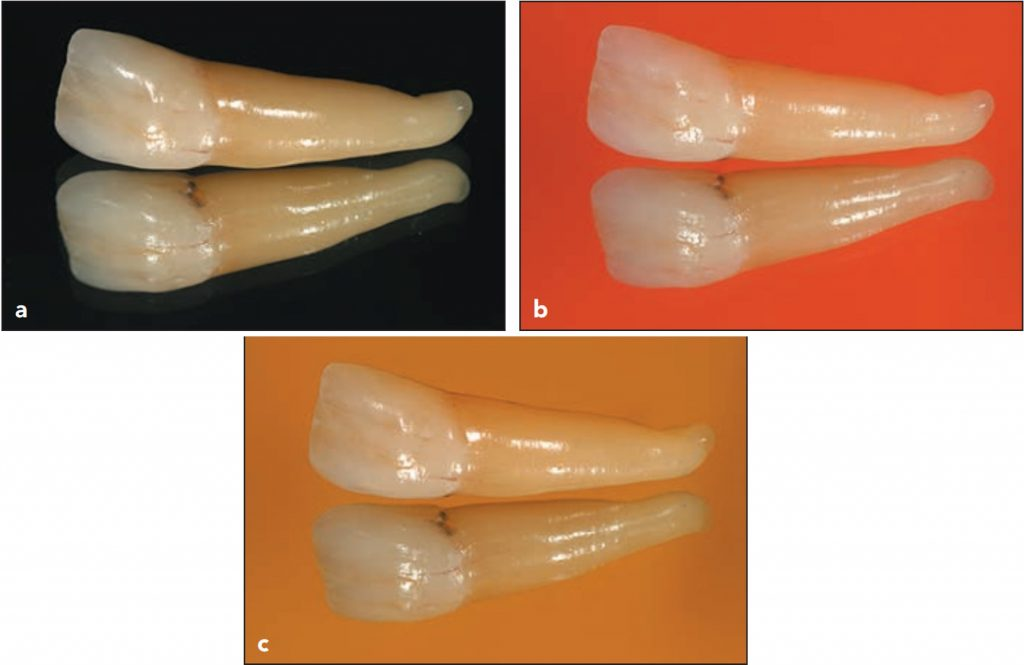
\includegraphics[width=0.7\columnwidth]{pictures/chroma.jpeg}
    \caption{a – màu răng không bị ảnh hưởng bởi chroma, b- nền màu đỏ-cam thì khó xác định màu hơn, c- nền màu vàng – cam còn khó xác định hơn nữa}
    \label{fig:chroma}
\end{figure}

\subsection{Hiệu ứng tương phản vùng khi so màu nha khoa}
\qquad Kích thước của vật thể cũng ảnh hưởng đến màu quan sát được, kích thước lớn hơn thì cảm nhận màu sáng hơn so với vật thể có kích thước nhỏ. Trong thực hành nha khoa, nếu răng có kích thước lớn thì màu chọn thường sẽ nên tối hơn so với mức bình thường vì cảm nhận màu của người quan sát sẽ thấy sáng hơn và ngược lại. Nếu răng hoặc miếng trám lớn thì nên tăng độ hue và ngược lại.\cite{TruongDinhKhoi}

\subsection{Hiệu ứng không gian khi so màu nha khoa}
\qquad Vật thể càng gần mắt người quan sát thì càng sáng hơn và lớn hơn, và ngược lại, càng ở xa thì càng nhỏ và tối hơn. Trong nha khoa, răng phía trước có xu hướng sáng hơn răng phía sau, răng chen chúc thì phía trước sáng hơn răng chen chúc phía sau. Vì vậy, bác sĩ nên giữ đồng nhất khoảng cách từ mắt đến răng so màu, và có kế hoạch bù trừ màu với răng thụt vào thì màu nên cho sáng hơn so với răng nhô ra so với cung hàm.\cite{TruongDinhKhoi}

%chèn ảnh không gian so màu
\begin{figure}[h]
\centering
    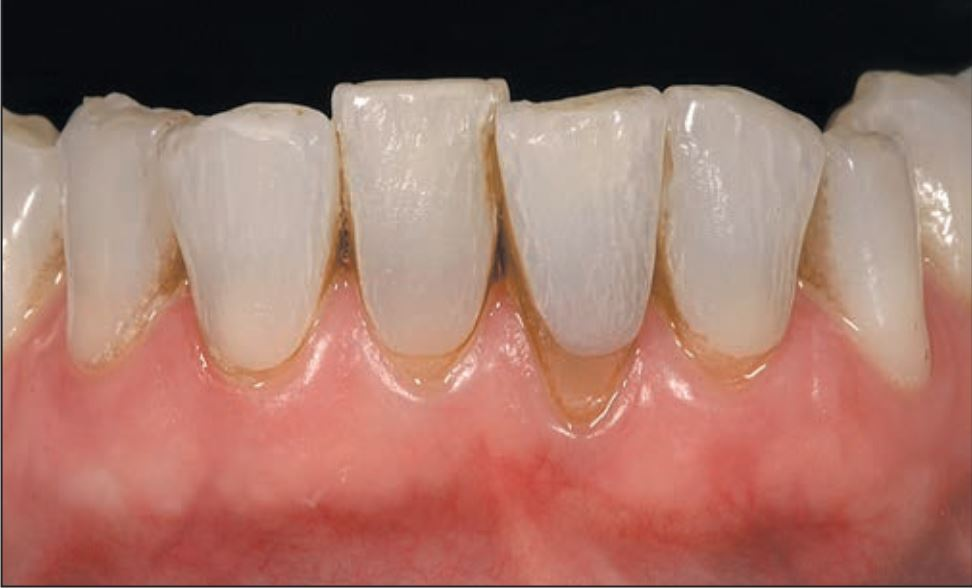
\includegraphics[width=0.7\columnwidth]{pictures/không gian so màu.jpeg}
    \caption{Răng 41 có vẻ tối hơn so với răng 31 do hiệu ứng không gian}
    \label{fig:không gian so màu}
\end{figure}

\subsection{Hiệu ứng tương phản dư ảnh khi so màu nha khoa}
\qquad Xảy ra khi vừa quan sát một màu trong một khoảng thời gian đủ lâu sau đó ngay lập tức quan sát một màu khác, màu quan sát trước đó sẽ dư ảnh và ảnh hưởng thành màu tương phản khi quan sát trên nền trắng. Có hai loại dư ảnh: Dư ảnh âm bản (tương phản màu thực) và dư ảnh dương bản (trở lại màu thực).\cite{TruongDinhKhoi}


\subsection{Nhận thức màu kém}
\qquad Những người có khiếm khuyết trong nhận thức màu sắc thì khó khăn trong việc xác định màu của vật thể, có thể kém nhận thức một hoặc nhiều màu, mức độ có thể từ nhẹ đến mức hoàn toàn không nhận thức màu sắc.\cite{TruongDinhKhoi}\par

%ảnh mù màu
\begin{figure}[h]
\centering
    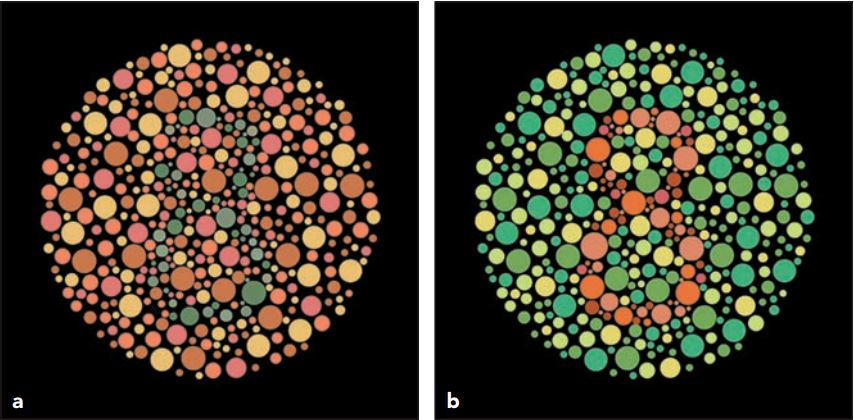
\includegraphics[width=0.8\columnwidth]{pictures/mù màu.jpeg}
    \caption{Bảng test màu a): test độ nhạy với màu xanh lá và màu vàng để phát hiện số 8; b): test ngược, số 8 dễ nhận thấy hơn với màu tím- đỏ}
    \label{fig:mù màu}
\end{figure}


\quad Khi bị khiếm khuyết về màu thì cảm nhận hue bị sai lệch so với chuẩn của người bình thường, giảm khả năng phân biệt màu, độ bão hoà hoặc độ sáng tối của màu.\cite{TruongDinhKhoi}

%ảnh mắt??
\begin{figure}[h!]
\centering
    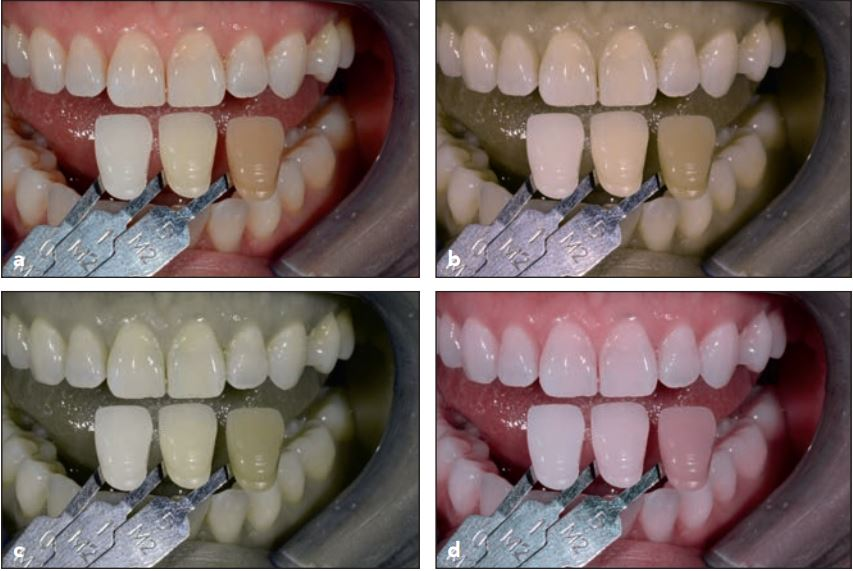
\includegraphics[width=0.8\columnwidth]{pictures/mắt.jpeg}
    \caption{a): Hình ảnh so màu của người bình thường, b): so màu của người mù màu đỏ, c): so màu của người mù màu xanh lá, d): so màu của người mù màu xanh dương}
    \label{fig:mắt}
\end{figure}

\subsection{Tuổi}
\qquad Tuổi ảnh hưởng đến kết quả so màu khi thuỷ tinh thể và giác mạc sẽ đục dần theo tuổi, có xu hướng nghiêng dần về màu vàng-nâu theo tuổi nên khó phân biệt hơn giữa mùa trắng và màu vàng. Quá trình giảm nhạy cảm màu sau tuổi 30 và rõ ràng khi bước sang tuổi 60, nhiều người ở tuổi 60 gặp khó khăn với màu tím và màu xanh dương.\cite{TruongDinhKhoi}

\subsection{Sức khoẻ thể chất của người quan sát}
\qquad Sự mệt mỏi có thể ảnh hưởng đến quá trình so màu, mệt mỏi ở mắt và toàn thân có sự ảnh hưởng khác nhau, khi mắt mệt mỏi thì người so màu có xu hướng thích nghi với màu sắc. Sự thích nghi phần lớn là điều chỉnh độ nhạy với màu sắc của các thụ thể nhận cảm. Sự nhận cảm của tế bào nón chia thành ba cặp màu đối lặp: xanh dương-vàng, đỏ-xanh lá, đen-trắng. Sự kích thích một màu bất kỳ sẽ gây ức chế các cặp còn lại, như vậy khi mắt mệt mỏi thì không thể đưa ra phán đoán chính xác về màu sắc, đặc biệt sau khi bị kích thích bởi một màu quá nhiều. Sự mệt mỏi toàn thân cũng gậy ra những sai lệch trong nhận thức màu sắc.\cite{TruongDinhKhoi}

 \subsection{Sự thích nghi ánh sáng và bóng tối của người quan sát}
 \qquad Sự thích nghi ánh sáng và bóng tối là khả năng ít bị nhạy cảm trước kích thích của màu sắc khi thay đổi về các đặc tính của màu như giá trị màu, độ sáng và độ bão hòa của màu. Có ba sự thích nghi ảnh hưởng đến nhận thức màu là thích nghi ánh sáng, bóng tối và màu sắc. Thích nghi với ánh sáng là sự giảm độ nhạy cảm của thị giác khi mức độ chiếu sáng tổng thể tăng lên. Ví dụ, khi bước vào căn phòng chiếu sáng tốt ngay sau khi rời khỏi căn phòng tối, thích nghi bằng cách ít nhạy cảm hơn, thường mất khoảng 5 phút để thiết lập hoàn toàn sự thích nghi này. Sự thích nghi bóng tối là quá trình ngược lại với thích nghi ánh sáng, trở nên nhạy cảm hơn với ánh sáng, thường mất khoảng 30 phút để thiết lập hoàn toàn. Sự thích nghi màu sắc là ít nhạy cảm khi có sự thay đổi màu sắc liên tục.\cite{TruongDinhKhoi}

 \subsection{Dinh dưỡng}
 \qquad Chế độ dinh dưỡng đóng một vai trò quan trọng đối với người so màu nói riêng và con người nói chung, trong đó vitamin A có vai trò ảnh hưởng trực tiếp đến thị lực, lượng vitamin A cần thiết mỗi ngày trong khoảng từ 900-3000 microgram (mcg)/ngày.\cite{TruongDinhKhoi}

\subsection{Cảm xúc}
\qquad Trạng thái cảm xúc của con người có ảnh hưởng đến quá trình xác định và đánh giá màu sắc, ngoài cảm xúc hoặc tâm trạng thì sở thích về màu sắc cũng có liên quan đến chọn lựa màu sắc. Do vậy, trong thực hành nha khoa, trước khi so màu, người quan sát cần thư giãn và mời thêm cộng sự so màu cùng để đưa ra những kết luận chính xác hơn.\cite{TruongDinhKhoi}

\subsection{Rối loạn nhận thức màu do thuốc}
\qquad Thuốc có thể thay đổi nhận thức về màu sắc do làm thay đổi về chất dẫn truyền thần kinh, thay đổi độ nhạy về màu do liên quan đến chuỗi phản ứng hóa học của các thụ thể võng mạc. Ví dụ, thuốc nhóm phosphodiesterase như sildenafil làm sai lệch nhận thức màu xanh dương. Thuốc điều hòa nhịp tim như amiodarone hoặc thuốc điều trị bệnh lao như ethambutol gây rối loạn màu sắc.\cite{TruongDinhKhoi}

\subsection{Sự khác biệt giữa hai mắt người quan sát}
\qquad Màu sắc được sự phối hợp và thống nhất giữa hai mắt khi cùng nhìn về vật thể, sự chênh lệch thị lực giữa hai mắt có thể gây ra những sai lệch khi so màu. Khi đặt hai vật thể giống nhau cạnh nhau thì thấy khác nhau về màu sắc, điều đó chứng tỏ hai mắt không tương đồng về cảm nhận màu sắc.\cite{TruongDinhKhoi} 

\subsection{Các đặc tính quang học của men và ngà}
\par 
\qquad Các thuộc tính của men/ngà ảnh hưởng đến nhận thức màu sắc của răng bao gồm độ trong/mờ (translucency/opacity), độ huỳnh quang (fluorescence), độ trắng đục (opalescence) và độ sáng bóng (gloss). Độ trong/mờ tuyệt đối gọi là transparency, cho ánh ánh sáng truyền qua hoàn toàn, không xảy ra hiện tượng phản xạ hay hấp thụ ánh sáng, tương ứng độ đục bằng 0. \cite{TruongDinhKhoi}

\textbf{
\section{Bảng so màu Vita 3D Master}}
\quad Bảng so màu Vita 3D Master được ký hiệu theo thứ tự số - chữ cái - số (ví dụ 3M2), trong đó thể hiện theo thứ tự giá trị của hue, value và chroma.\cite{TruongDinhKhoi} Theo thứ tự value, chia thành sáu nhóm có giá trị value giảm dần từ nhóm 0 đến nhóm 5:\par
\quad \textit{Nhóm 0:} Nhóm có value cao nhất, chỉ có một hue ký hiệu M (màu trung tính) có 3 cây 0M1, 0M2, 0M3 theo thứ tự tăng dần chroma từ nhạt đến sẫm màu hơn 0M1<0M2<0M3.\par
\quad \textit{Nhóm 1:} 2 cây 1M1 và 1M2, có cùng hue màu trung tính ký hiệu M, có thứ tự tăng dần chroma 1M1<1M2.\par
\quad \textit{Nhóm 2, 3 và 4:} Có 7 cây, chia thành 3 phân nhóm nhỏ theo thứ tự thay đổi hue gồm: nhóm L (left) - màu vàng, nhóm M (medium) - màu trung tính, nhóm R (right) - màu đỏ. Trong nhóm L, độ chroma tăng dần 2L1<2L2; 3L1<3L2; 4L1<4L2. Trong nhóm M, độ chroma tăng dần 2M1<2M2<2M3; 3M1<3M2<3M3; 4M1<4M2<4M3. Trong nhóm R, độ chroma tăng dần 2R1<2R2; 3R1<3R2; 4R1<4R2.\par
\quad \textit{Nhóm 5:} Có 3 cây, nhóm có value thấp nhất, chỉ có một hue ký hiệu M tương tự nhóm 0 (màu trung tính), 3 cây gồm 5M1, 5M2, 5M3 theo thứ tự tăng dần chroma 5M1<5M2<5M3.\par

%chèn ảnh bảng so màu vào đây nháaa
\begin{figure}[h]
\centering
    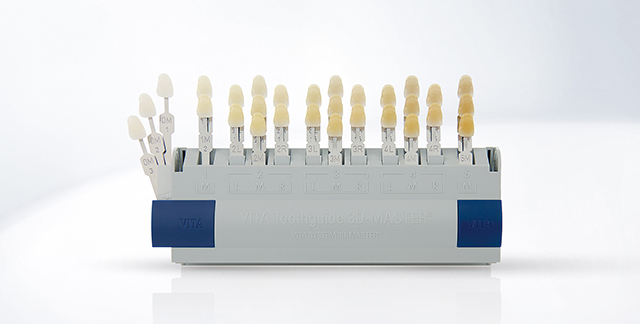
\includegraphics[width=0.7\columnwidth]{pictures/anh-vita-3d.jpeg}
    \caption{Bảng so màu Vita 3D Master}
    \label{fig:anh-vita-3d}
\end{figure}

\quad \textbf{Các bước so màu sử dụng bảng màu Vita:}\par
\quad \textit{Bước 1: }Chọn value, chọn một trong sáu nhóm sao cho độ sáng của răng giống nhất với độ sáng của các cây loại M trong bảng so màu từ nhóm value đã chọn được.\par
\quad \textit{Bước 2:} Chọn chroma, từ các cây loại M đã chọn xác định cây có chroma gần giống nhất với răng được so màu.\par
\quad \textit{Bước 3:} Chọn hue, từ các cây có cùng value và chroma, so sánh với các cây loại L và R có cùng value và chroma với cây loại M vừa chọn, từ đó chọn ra cây có hue gần giống nhất với răng so màu, viết ký hiệu màu chọn theo quy ước của bảng so màu.
\vspace{5pt}
\textbf{
\section{Các nguyên tắc khi so màu}}
\quad Trước khi so màu cần đảm bảo đủ tiêu chuẩn về nguồn sáng, lý tưởng nhất dưới ánh sáng tự nhiên và đủ tiêu chuẩn kỹ thuật trên. Loại bỏ màu sắc gây nhiễu xung quanh răng so màu, tránh sử dụng màu sắc khác gây nhiễu loạn và mỏi mắt trước và trong khi so màu.\cite{TruongDinhKhoi}\par

\quad Vị trí đặt bảng so màu phụ thuộc vào phương pháp so màu và mục đích so màu, so màu pha macro thì đặt bảng so màu, sau đó chọn các cây tiếp tục cho pha sau như pha mini và pha micro.\par

\quad Có thể đặt giữa răng hàm trên và hàm dưới hoặc kế bên ngang mức rìa cắn răng cần so màu, tránh đặt chồng lên phía trước hoặc phía sau răng cần so màu\par

%ảnh nguyên tắc so màu 
\begin{figure}  [h]
    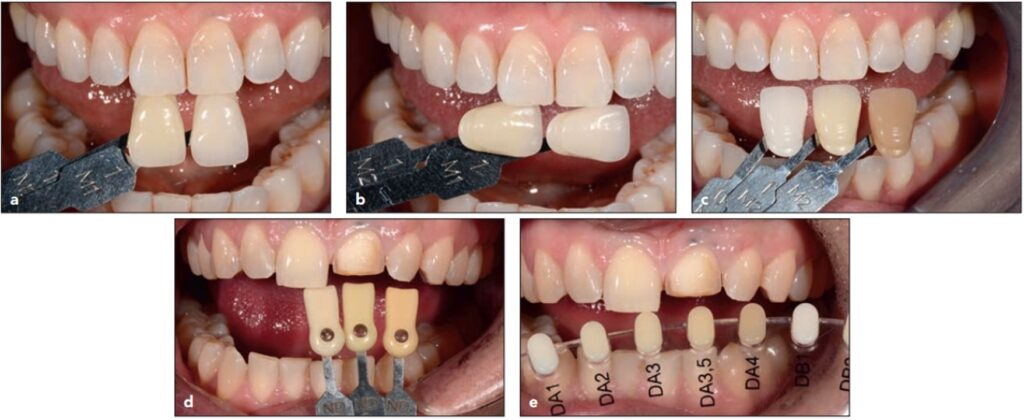
\includegraphics[width=1\columnwidth]{pictures/nguyên tắc so màu.jpeg}
    \caption{a): đặt cổ - rìa cắn, b): đặt nằm ngang, c): đặt đối đầu, d và e): so màu cùi răng}
    \label{fig:nguyên tắc so màu}
    \end{figure}
    
\quad Phương pháp so màu theo mô hình ba pha macro - mini - micro, bắt đầu bằng pha macro bằng cách sử dụng toàn bộ bảng so màu, chọn và đặt sang một bên các màu được lựa chọn để dùng cho pha sau, loại bỏ các màu không phù hợp. Ở pha mini, các cây được lựa chọn thì chọn tiếp sao cho phù hợp về màu của cổ, thân và rìa cắn gần nhất với răng cần so màu. Ở pha micro thì so sánh chi tiết về hue, value và chroma. Không đặt rìa cắn hướng về phía kim loại của bảng so màu.\par
\quad Nên so màu răng cả cùi răng và so màu từng phần của răng thành ba phần rìa cắn, thân và cổ răng. Kết quả so màu cần ghi ký hiệu màu dưới dạng “ngôn ngữ màu (color language)” theo từng loại bảng so màu của nhà sản xuất nhằm thống nhất màu giữa bác sĩ và labo răng.\par
\vspace{-5pt}
\textbf{
\section{Các phương pháp so màu}}
\quad Hiện nay có nhiều phương pháp đánh giá màu răng như sử dụng bảng so màu băng giấy, sứ có màu hoặc nhựa acrylic, sử dụng quang phổ kế, sắc kế và kỹ thuật phân tích hình ảnh.\cite{NguyenThiChau}\par
\quad Việc xác định màu bằng cách so màu răng với màu răng mẫu trên bảng so màu là ứng dụng phổ biến nhất trong nha khoa. Răng và bảng so màu được quan sát cùng lúc dưới điều kiện ánh sáng như nhau. Ánh sáng bên ngoài, kinh nghiệm, tuổi, sự mỏi mắt và vấn đề sinh lý (mù màu) có thể dẫn tới mâu thuẫn và sai lệch. Mặt khác tiêu chuẩn hóa thuộc tính màu sắc được đánh giá bằng thị giác bị giới hạn. Theo Joiner (2004), màu cơ bản của một răng được xác định ở một phần ba giữa răng bởi vì dải màu thay đổi từ rìa cắn tới viền lợi và quan sát viên phải tập trung vào vùng này. \par
\quad Xác định màu bằng quang phổ kế: Theo Andjelkovic (2010) và Lenhmann (2010) là đo một độ dài bước sóng tại thời điểm từ khi truyền ánh sáng của một đối tượng và được sử dụng để đo quang phổ hữu hình của những răng đã nhổ và răng sống. Theo Corciolani (2007), sử dụng quang phổ kế đo màu sắc là chính xác nhất.\cite{NguyenThiChau}	\par	
\quad Sắc kế có bộ lọc màu xấp xỉ chức năng quang phổ của mắt quan sát viên đạt tiêu chuẩn và được đo màu trong 3 nhóm màu cơ bản trong hệ thống màu CIE L, a*, b*. Phép đo bằng sắc kế đã được so sánh với sự ghi quang phổ kế là đáng tin cậy và chính xác để đo lường màu sắc.\cite{NguyenThiChau}\par
\vspace{-5pt}
\textbf{
\section{Chỉ số nhu cầu điều trị làm trắng răng}}
\quad Khi xây dựng chỉ số nhu cầu điều trị tẩy trắng răng, điều quan trọng là phải xem xét nhu cầu điều trị dựa trên nhiều tình huống bao gồm các vấn đề bẩm sinh như khuyết tật di truyền của răng hoặc khuyết tật bẩm sinh như mảng trắng hoặc nâu.\cite{LindaGreenwall2019}\par
\quad Theo Whitening Group, giới hạn được thiết lập bởi các quy định hiện hành gây khó khăn cho việc điều trị bệnh nhân một cách dễ dàng và tiết kiệm chi phí; tuy nhiên, những người có các chỉ định sau nên được ưu tiên\cite{LindaGreenwall2019}:\par
\begin{enumerate}
    \setlength{\itemsep}{0pt}
    \item Sự đổi màu nghiêm trọng và trung bình.
    \item Điều kiện tráng men.
    \item Đốm trắng và vết trắng nhỏ.
    \item Nhuộm màu nâu, cam và vàng.
    \item Khiếm khuyết về mặt thẩm mỹ.
    \item Răng cửa mọc lệch lạc.
    \item Thiểu sản răng cửa hàm.
    \item Chấn thương.
    \item Yếu tố di truyền, ví dụ: sự tạo men răng bất toàn.
    \item Có răng trước bị đổi màu không còn sức sống.
\end{enumerate}
\par
\quad Các cân nhắc khác nhau được đưa ra khi đánh giá các chỉ định cho nhu cầu điều trị\cite{LindaGreenwall2019}:\par
\begin{itemize}
\setlength{\itemsep}{0pt}
    \item Sắc thái của sự đổi màu (ví dụ: các sắc thái rất đậm—A4, C4, B4): sự đổi màu như vậy (dấu hiệu 1) được chia thành nghiêm trọng, trung bình và nhẹ. Điều trị tẩy trắng nên được thực hiện nếu loại đổi màu có thể được xếp vào loại nghiêm trọng hoặc trung bình, trẻ nhận thức được sự đổi màu và sự đổi màu có ảnh hưởng đến cuộc sống của trẻ.
    \item Tính chất và mức độ biến màu.
    \item Sự đổi màu có lan rộng trên răng hay không hoặc có lốm đốm trên răng hay không.
    \item Răng có màu sắc bình thường nhưng có vết trắng, lốm đốm hoặc vệt trắng.
    \item Sự hiện diện của sự đổi màu nâu trên bề mặt môi trong của răng, có thể do chấn thương (chảy máu vào răng trước đó) hoặc dấu hiệu nhiễm fluorosis. Đôi khi không rõ nguyên nhân. \item Thông thường, phần đổi màu nâu sẽ được loại bỏ đầu tiên khi quá trình điều trị làm trắng bắt đầu và là phần làm sáng nhanh nhất. Đôi khi có thể mất nhiều thời gian hơn để điều trị làm trắng loại bỏ hoàn toàn đốm nâu. Nó có thể mờ dần thành một vết màu vàng nhạt. Khi màu nền được làm sáng, dấu hiệu sẽ ít được chú ý hơn. Các vết đổi màu nâu có thể được loại bỏ khoảng 80\% thời gian (Haywood 2006). Chỉ có một số vùng màu nâu cần xử lý lại sau 1-3 năm (Haywood 2006).
    \item Xuất hiện các mảng trắng trên răng cửa và răng hàm. Ngày càng có nhiều đốm trắng trên răng. Các đốm và mảng trắng có thể lan rộng trên các răng trước cũng như các răng hàm đầu tiên. Nếu có tình trạng này thì chỉ định can thiệp phục hồi răng hàm sớm cũng như điều trị tẩy trắng răng để giảm ảnh hưởng của các vết trắng trên bề mặt môi trong của răng.
    \item Ảnh hưởng của sự đổi màu đối với trẻ.
    \item Sự đổi màu có dễ dàng được tẩy trắng hay có thể yêu cầu nhiều lựa chọn xử lý như tẩy trắng, xử lý bề mặt men răng như xử lý Sylc, phun cát, mài mòn siêu nhỏ (12–26 micron men được loại bỏ sau 5 giây sử dụng; Haywood 2006), hoặc xâm nhập nhựa.
    \item Liệu có sự đổi màu răng đơn lẻ chẳng hạn như răng chết do chấn thương hay không.
    \item Có nhiều vết đổi màu trên toàn bộ răng hay không. Bệnh nhân với các điều kiện được đề cập bởi Nhóm làm việc nên được điều trị với kế hoạch điều trị thích hợp theo chẩn đoán.
\end{itemize}

\quad \textbf{Chỉ số về nhu cầu điều trị tẩy trắng răng cho bệnh nhân dưới 18 tuổi:}\cite{LindaGreenwall2019}\par
\textbf{Loại 1 - Cao}
\begin{enumerate}
\setlength{\itemsep}{0pt}
    \item Sự đổi màu: nghiêm trọng
    \item Vị trí vết: phân bố nhiều đậm nhạt đồng đều
    \item Ảnh hưởng đến trẻ em: nghiêm trọng
    \item Nhu cầu làm trắng: cao
\end{enumerate}

\textbf{Loại 2 - Trung bình}
\begin{enumerate}
\setlength{\itemsep}{0pt}
    \item Sự đổi màu: vừa phải
    \item Vị trí: phân bố đều
    \item Ảnh hưởng đến đứa trẻ: có ảnh hưởng đến đứa trẻ
    \item Nhu cầu làm trắng: vừa phải
\end{enumerate}

\textbf{Loại 3 — Mong muốn}
\begin{enumerate}
\setlength{\itemsep}{0pt}
    \item Sự đổi màu: nhẹ
    \item Vị trí: ít răng trước
    \item Tác động đến trẻ em: một số tác động
    \item Nhu cầu làm trắng: mong muốn; điều này sẽ dễ dàng làm giảm bớt các vấn đề đổi màu
\end{enumerate}

\textbf{Loại 4 — Khuyến cáo}
\begin{enumerate}
\setlength{\itemsep}{0pt}
    \item Sự đổi màu: các khu vực bị đổi màu bị cô lập
    \item Vị trí: phân bố ngẫu nhiên trên răng
    \item Ảnh hưởng đến trẻ em: vừa phải
    \item Nhu cầu làm trắng: khuyến cáo
\end{enumerate}

\textbf{Loại 5 — Có thể}
\begin{enumerate}
\setlength{\itemsep}{0pt}
    \item Sự đổi màu: đổi màu nhẹ hoặc đốm trắng
    \item Vị trí: ít răng hoặc một răng
    \item Ảnh hưởng đến trẻ em: không ảnh hưởng đến trẻ em
    \item Nhu cầu làm trắng: có thể thực hiện được; có thể được mong muốn, nhưng có thể đợi cho đến khi đứa trẻ trên 18 tuổi.
\end{enumerate}
\vspace{-5pt}
\textbf{
\section{Các nghiên cứu trên thế giới và Việt Nam về màu sắc răng và nhu cầu làm trắng răng}}
\subsection{Trên thế giới}
\qquad Trong bài viết “Dental Whitening: Self-Referred Needs versus Professional Indication” của Renata Pedrosa Guimarães (2021) đã có những thảo luận như sau:\par
\quad Về các câu hỏi liên quan đến tẩy trắng răng, đáng chú ý là: chỉ có 15,5\% trả lời khẳng định là đã thực hiện tẩy trắng răng rồi. Trong số này, 6,9\% đã trải qua tẩy trắng răng bằng cách sử dụng kỹ thuật tại phòng khám, 5,2\% đã trải qua quá trình làm trắng có giám sát và một cá nhân đã sử dụng thuốc không kê đơn sọc trắng. Đa số (63,8\%) cho biết cần tẩy trắng răng trong câu hỏi về ai hoặc cái gì đưa ra các tiêu chuẩn liên quan đến màu sắc lý tưởng của nụ cười, hơn một nửa (56,9\%) đã trả lời rằng đó là “Phương tiện truyền thông”, tiếp theo là 19,0\% là “Lòng tự trọng” và 10,3\% cho rằng đó là “Xã hội”.\cite{Renata2021} \par
\quad Sự so sánh giữa tần suất học sinh đã tẩy trắng răng theo độ tuổi và giới tính, nơi có thể quan sát thấy tỷ lệ đã trải qua răng nhóm tuổi từ 20 đến 46 làm trắng cao hơn so với nhóm tuổi từ 18 đến 19 (22,2\% so với 9,7\%) và điều này tỷ lệ phần trăm chỉ cao hơn 1,3\% ở nữ (16,1\% so với 14,8\%), tuy nhiên đối với biên độ sai số của thống kê kiểm tra (5\%) không có mối liên hệ đáng kể nào giữa câu hỏi với bất kỳ biến nào trong hai biến được phân tích (p>0,05).\cite{Renata2021}\par
\quad Trong nghiên cứu về câu hỏi "Bạn có nghĩ rằng bạn cần phải làm trắng răng?" Tỷ lệ trả lời khẳng định là: nữ cao hơn nhiều so với nam (p=0,001). Các câu trả lời là khẳng định đối với hầu hết sinh viên trong tất cả các khóa học, ngoại trừ những người trong các khóa học y khoa, với sự nhấn mạnh về dinh dưỡng học sinh (70,0\%) và học thể dục (63,6\%). Sự liên kết giữa câu hỏi là
kiểm chứng cho cả hai biến (p<0,05). Tám (88,9\%) trong số chín cá thể được chụp ảnh có màu tối hơn trên thang đo so với màu thực tế được hiển thị bởi máy đo quang phổ kỹ thuật số. Chỉ dành cho một trong số họ (11,1\%), các giá trị này trùng nhau.\cite{Renata2021}\par
\quad Kết quả của 180 đánh giá được thực hiện bởi 20 nha sĩ ở chín cá nhân ai nói cần tẩy trắng, tùy chuyên ngành, thời gian tốt nghiệp và giảng dạy cơ sở giáo viên đã tham gia khóa học. Từ bảng này, có thể nhấn mạnh rằng: hơn một nửa (53,9\%) câu trả lời là tẩy trắng răng; có một mối liên quan đáng kể giữa chỉ định của làm trắng với chuyên ngành và thời gian kể từ khi ra trường. Tỷ lệ các dấu hiệu tích cực cao hơn trong số bác sỹ thuộc các chuyên khoa: Răng Hàm Mặt, Răng Hàm Mặt + Chỉnh Nha và Răng Hàm Mặt + Cấy Ghép Implant, và thấp hơn giữa các chuyên khoa Răng Hàm Mặt + Nội Nha, Nội Nha, Nhi Khoa và Nha Chu. Cao nhất phần trăm phản hồi có chỉ định tẩy trắng xảy ra ở những người có hơn 20 năm tốt nghiệp (65,3\%) và thấp nhất là nhóm từ 10 đến 19 tuổi (35,6\%).\cite{Renata2021}\par
\quad Hiện nay, các chuyên gia và bệnh nhân chia sẻ lý tưởng thẩm mỹ liên quan trực tiếp đến răng nhẹ. Các nhận thức về những gì là thẩm mỹ hoặc không thẩm mỹ, liên quan đến màu sắc của răng, thay đổi tùy thuộc vào bối cảnh của hiệu suất của mỗi người, bệnh nhân và các chuyên gia. Ý kiến về màu sắc của răng có một cực kỳ tính chất chủ quan và rất khác nhau giữa chuyên gia này và chuyên gia khác. Đa số bệnh nhân tự nhận thấy màu răng của họ tối hơn so với thực tế. Bệnh nhân nữ thường mong muốn có hàm răng sáng màu hơn.\cite{Renata2021}\par
\quad Cuối cùng, phương tiện truyền thông có vai trò quyết định trong việc xác định tiêu chuẩn thẩm mỹ của nụ cười.\par
\subsection{Ở Việt Nam}
\qquad Trong “Nghiên cứu hiệu quả điều trị tẩy trắng răng sống Tetracycline" của Nguyễn Thị Châu (2013) cho thấy phân bố màu sắc nhóm răng theo phổ màu Munsell: Điểm màu Vita V, độ bão hòa màu C: Cao nhất là răng nanh và thấp nhất là răng hàm nhỏ, sự khác biệt có ý nghĩa thống kê. Tông màu h: Răng nanh thấp nhất và răng hàm nhỏ là cao nhất, sự khác biệt có ý nghĩa thống kê. \par
\quad Bảng Vita cổ điển chia làm 4 nhóm màu: Nhóm A đặc trưng cho màu vàng đỏ hoặc nâu đỏ, nhóm B đặc trưng cho màu vàng, nhóm C đặc trưng cho màu xám, nhóm D đặc trưng cho màu vàng ánh đỏ theo thang điểm độ sáng tối. Màu sắc ở răng cửa (tương ứng B4) có màu vàng nâu xám nhẹ. Răng nanh (tương ứng C4 - A4) có màu vàng xám đỏ. Răng hàm nhỏ tương ứng B3 - A3.5 có màu vàng cam đỏ. Theo tông màu h xác định màu sắc trên tọa độ cực răng nanh (75,9) tương ứng màu vàng xám đỏ, răng cửa (79,4) tương ứng vàng đỏ và răng hàm nhỏ (81,7) tương ứng vàng cam, cũng tương đồng với điểm màu Vita\cite{NguyenThiChau}. \par
\quad Như vậy, màu sắc răng không đồng nhất giữa nhóm răng cửa, nanh và răng hàm nhỏ, trong đó nhóm răng phía trước màu đậm hơn so với răng phía sau, sự khác biệt có ý nghĩa thống kê. Điểm màu Vita của răng hàm nhỏ là thấp nhất, sau đó đến răng cửa, cuối cùng là răng nanh. Ngoài ra độ bão hòa màu của răng nanh là cao nhất, thấp nhất là răng hàm nhỏ.\cite{NguyenThiChau}\par


